\subsection{Periodo di Validazione e collaudo}
\subsubsection{MPC01 - SPICE}
Ogni sigla presente in questa sezione fa riferimento a quanto descritto all'interno del documento \textit{NormeDiProgetto-v3.0.0} §A\newline \newline
Data la brevità del periodo, gli unici processi che salgono di livello sono quelli di fornitura e gestione della configurazione. Nonostante questo tutti i processi raggiungono la soglia di accettazione.


\begin{table}[H]
    \rowcolors{2}{gray!25}{white}
    \rowcolors{2}{gray!25}{white}
        \renewcommand{\arraystretch}{1.5}
        \begin{tabular}{ m{0.15\textwidth}<{\centering}  m{0.055\textwidth}<{\centering} m{0.055\textwidth}<{\centering} m{0.055\textwidth}<{\centering} m{0.055\textwidth}<{\centering} m{0.055\textwidth}<{\centering} m{0.055\textwidth}<{\centering} m{0.055\textwidth}<{\centering} m{0.055\textwidth}<{\centering} m{0.055\textwidth}<{\centering} m{0.08\textwidth}<{\centering}}
	\rowcolor{darkblue}
	\textcolor{white}{\textbf{Processo}} &\textcolor{white}{\textbf{1.1}} &\textcolor{white}{\textbf{2.1}} &\textcolor{white}{\textbf{2.2}} &\textcolor{white}{\textbf{3.1}} &\textcolor{white}{\textbf{3.2}} &\textcolor{white}{\textbf{4.1}} &\textcolor{white}{\textbf{4.2}} &\textcolor{white}{\textbf{5.1}} &\textcolor{white}{\textbf{5.2}} &\textcolor{white}{\textbf{Livello}}\\ 


    Fornitura & F & F & F & F & F & N & N & N & N & 3 \\
    Sviluppo & F & F & F & F & F & N & N & N & N & 3 \\
    Documentazione & F & F & F & L & L & N & N & N & N & 2 \\
    Gestione della configurazione & F & F & F & F & F & N & N & N & N & 3 \\
    Gestione della qualità & F & F & F & F & F & N & N & N & N & 3 \\
    Verifica & F & F & F & L & P & N & N & N & N & 2 \\
   
    Gestione di processo & F & F & F & P & P & N & N & N & N & 2 \\
    Formazione dei membri del team & F & F & F & N & N & N & N & N & N & 2 \\
    
\end{tabular}       
\caption{Validazione e collaudo: MPC01 - SPICE}
\end{table}

\begin{figure}[H]
    \centering
    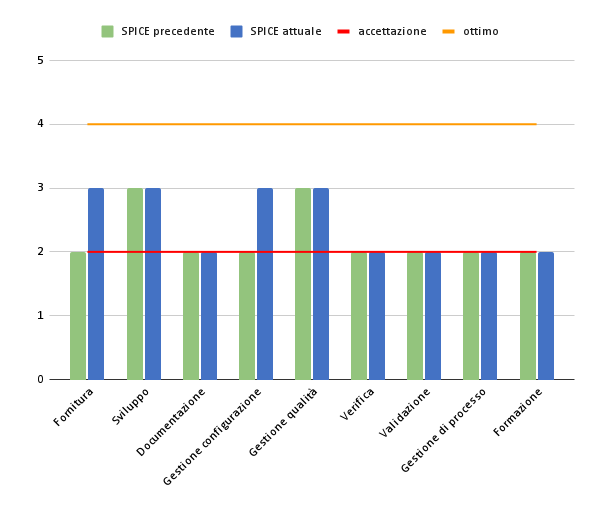
\includegraphics[scale=0.50]{Sezioni/images/vc-spice.png}
    \caption{Validazione e collaudo: MPC01 - SPICE}
\end{figure}

\subsubsection{MPC02 - BCWS}
\begin{figure}[H]
    \centering
    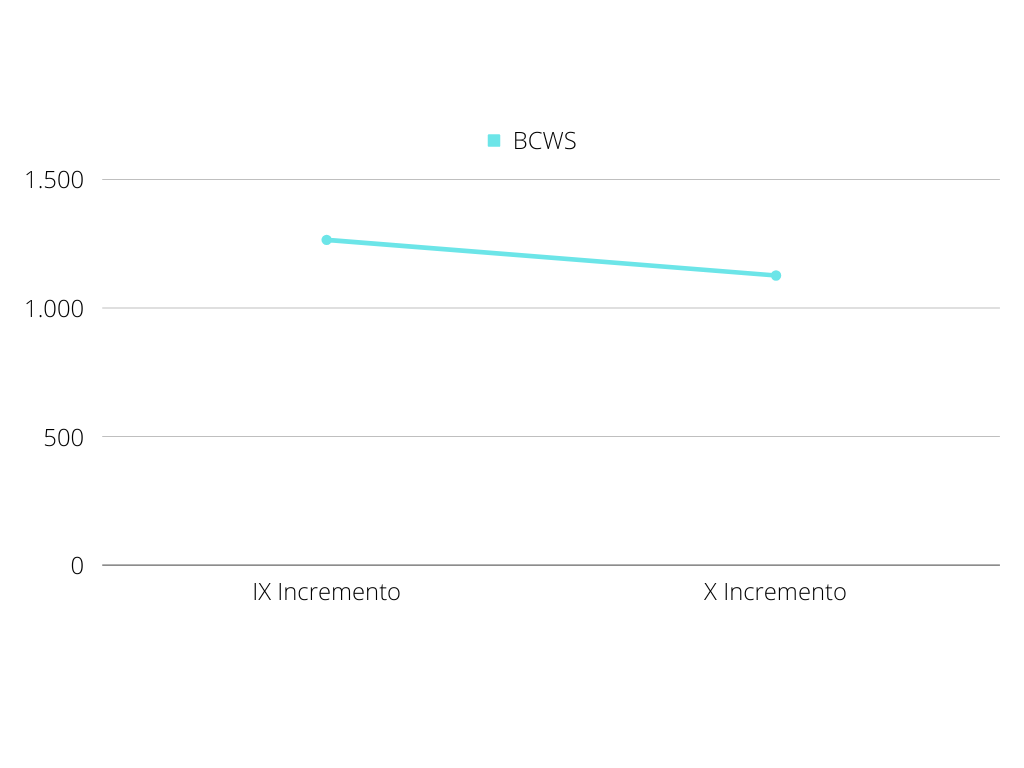
\includegraphics[scale=0.50]{Sezioni/images/vc-BCWS.png}
    \caption{Validazione e collaudo: MPC02 - BCWS}
\end{figure}

\subsubsection{MPC03 - ACWP}
\begin{figure}[H]
    \centering
    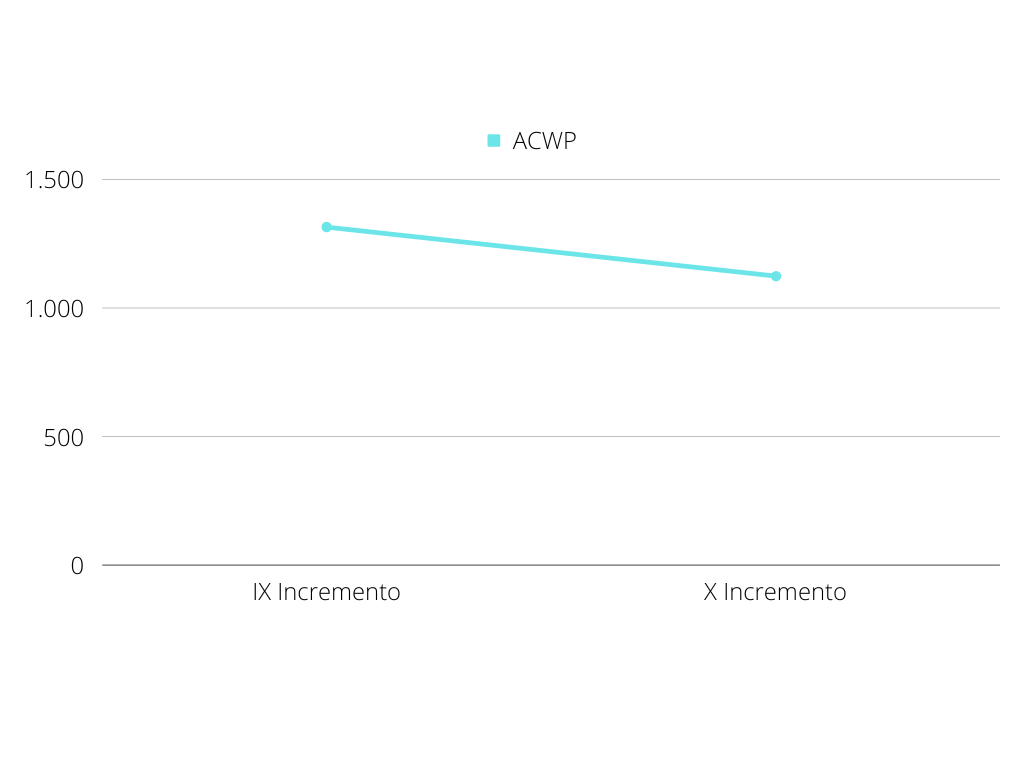
\includegraphics[scale=0.50]{Sezioni/images/vc-ACWP.png}
    \caption{Validazione e collaudo: MPC03 - ACWP}
\end{figure}

\subsubsection{MPC04 - BCWP}
\begin{figure}[H]
    \centering
    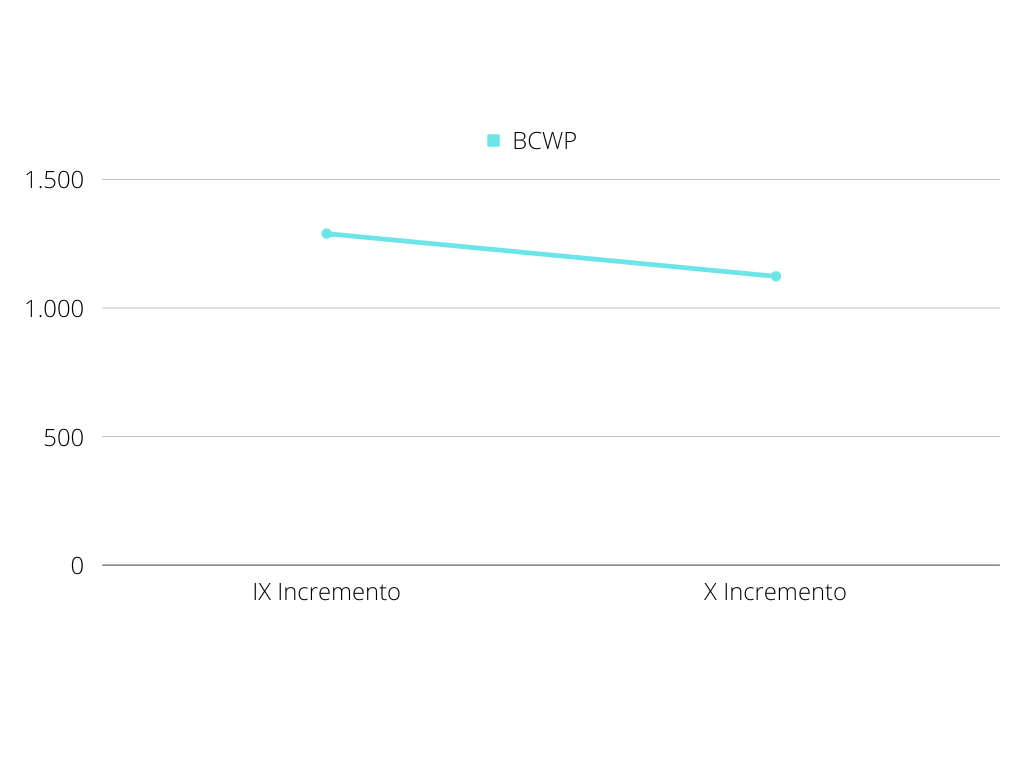
\includegraphics[scale=0.50]{Sezioni/images/vc-BCWP.png}
    \caption{Validazione e collaudo: MPC04 - BCWP}
\end{figure}

\subsubsection{MPC05 - Schedule variance}
La Schedule variance raggiunge un valore ottimo in entrambi gli incrementi.
\begin{figure}[H]
    \centering
    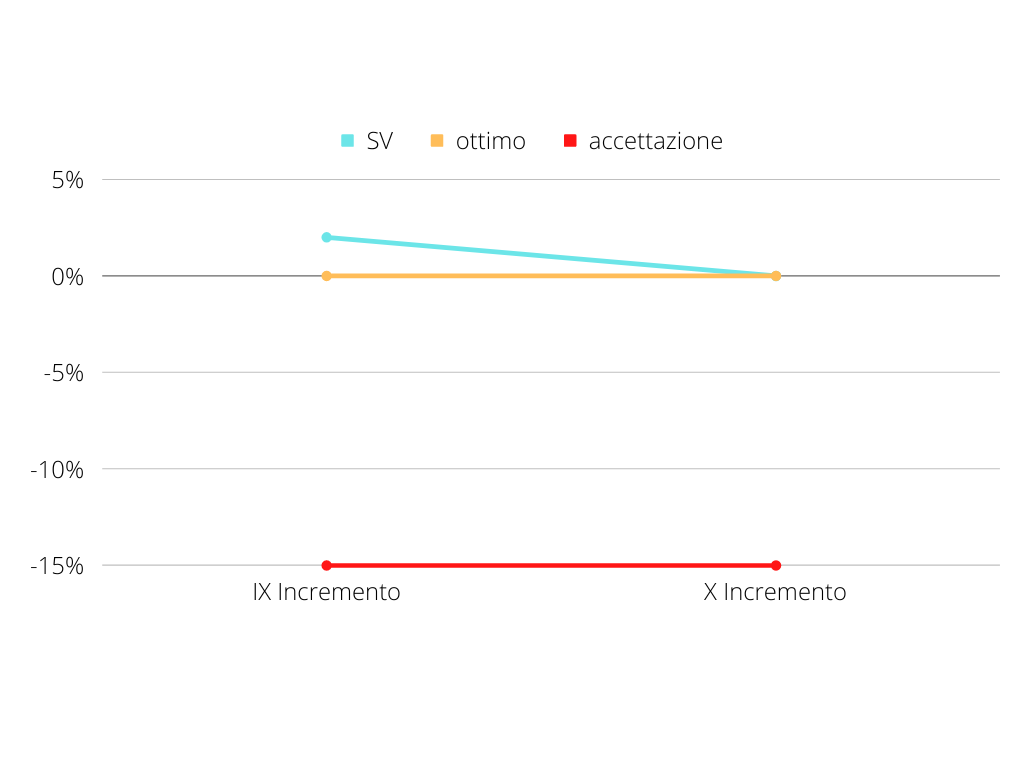
\includegraphics[scale=0.50]{Sezioni/images/vc-SV.png}
    \caption{Validazione e collaudo: MPC05 - SV}
\end{figure}

\subsubsection{MPC06 - Budget variance}
La Budget variance raggiunge un valore accettabile nel IX incremento ed un valore ottimo nel X incremento.
\begin{figure}[H]
    \centering
    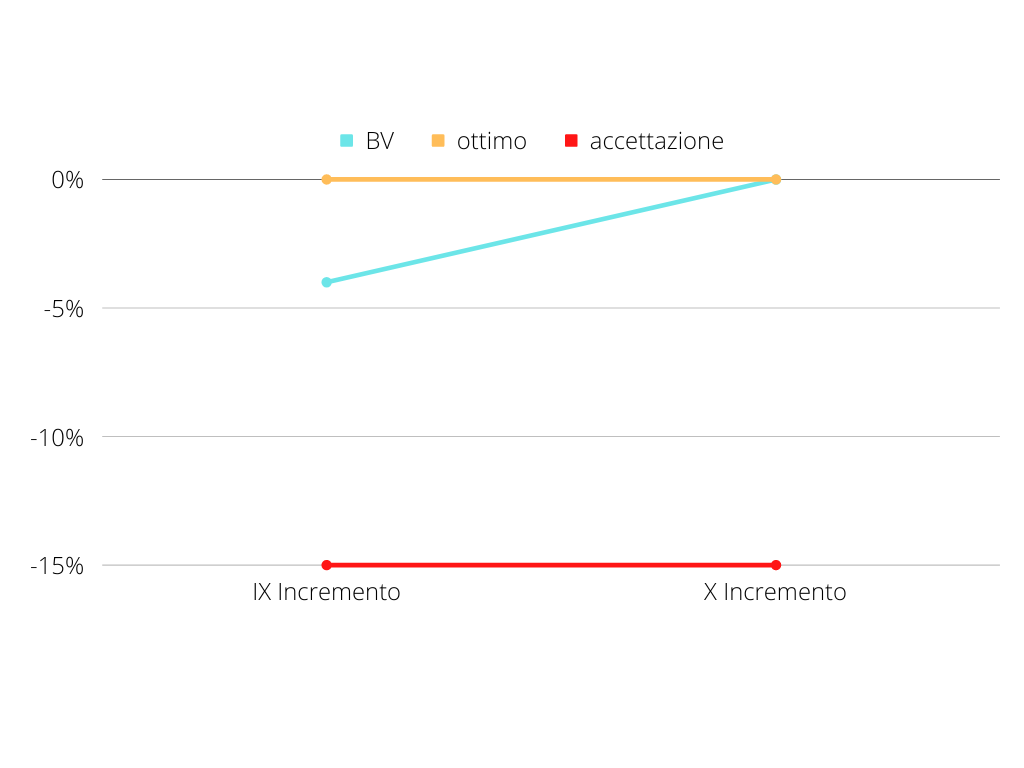
\includegraphics[scale=0.50]{Sezioni/images/vc-BV.png}
    \caption{Validazione e collaudo: MPC06 - BV}
\end{figure}